\chapter{Numerical Characterization of Quasi-Static Ultrasound Elastography}
	\label{chap:quasi-static}
	\section{Introduction}
		The goal of this study was to numerically characterize various important parameters related to detecting DTI using quasi-static ultrasound elastography (such as lesion geometry, material properties, and transducer characteristics) in order to examine the feasibility of using the technique to detect early DTI in humans. Quasi-static ultrasound elastography involves displacing the surface of the skin such that internal tissues are placed under a strain field. Ultrasound signals are used to track internal strains which then relate to the localized mechanical stiffness of the tissue---local regions that are significantly more or less stiff than surrounding tissue may be classified as either undergoing rigor mortis or necrosis and may present cause for concern.
		
	\section{Method}
		\label{sec:method}
		In order to evaluate the sensitivity of using quasi-static ultrasound elastography to detect deep tissue injuries, a numerical model of these injuries was created such that a subset of the investigated cases mimicked a physical phantom model which was used for validation. This numerical model allowed the rapid modification of numerous parameters related to DTI to examine their effect on the method's detection sensitivity where detection sensitivity is defined as the slope of the given characterization plot. An ideal detection sensitivity would resemble a unary mapping between the measured lesion stiffness ratio and the true lesion stiffness ratio. Lesions are considered to be ``detectable'' when the measured strain ratio of the lesion is significantly greater than or less than 1. Lesions with measured strain ratios of 1 would appear the same as healthy tissue and would most likely not be detected in the elastogram. To fully understand the problem, 5 general model cases were studied with each case generating numerous sub-studies on the effect of various parameters relating to that case. These parameters included: lesion depth; lesion altitude (distance of the lesion above deep bone); lesion diameter; ratio of the stiffness between the lesion and the surrounding tissue; ultrasound probing frequency; strain level applied by the transducer; the separation distance between two co-located lesions; radius of a circular averaging filter applied to the lesion boundaries; the number of smaller clustered lesions per unit area---noting that the small lesions in this model may overlap each other; the radius of each individual clustered lesion; the width of the lesion in a Visible Human \cite{visiblehuman} model and the depth of the lesion in a Visible Human model. The range of values for the tested parameters are given in Table \ref{tab:parametervalues} which resulted in a total of 144 model cases that were analyzed. The geometry of the models shown in Fig. \ref{fig:geometry} include: a cross-section of a simple spherical lesion embedded within a 2-dimensional rectangular zone of soft tissue; two lesions located at the same depth separated laterally by a finite dimension, $\delta_{sep}$; a cross-section of a spherical lesion without hard boundaries; a cluster of small lesions which together form a larger lesion area; and a lesion with mri-acquired geometry \cite{solis13} embedded in geometry obtained from a Visible Human slice \cite{visiblehuman}.

		In Fig. \ref{fig:schematic_human}, the lesion is located superficial to the left ischial tuberosity in the transverse plane. The lesion geometry was obtained from an MRI scan of a real deep tissue injury induced in a porcine model \cite{solis13}. The generic soft tissue in this model is modelled after muscle, with a layer of adipose tissue residing at the surface of the model.

		Note that the axial direction referred to henceforth as the ``axial'' direction of an ultrasound transducer placed along the top (superficial) surface of the domain such that it becomes the ``vertical'' direction.

		\begin{table}[!t]
			\centering
			\caption{Range of values of investigated parameters}
			\label{tab:parametervalues}
			\begin{tabular}{lcc}
				\toprule
				Parameter & Symbol & Values \\
				\midrule
				Lesion depth & $d$ & $[3.5, 6.5, 8.5, 10.0]$\,\si{\cm} \\
				Lesion altitude & $h$ & $[1.25, 2.50, 3.75]$\,\si{\cm} \\
				Lesion diameter & $\diameter S$ & $[0.5, 1.0, 2.0, 2.5]$\,\si{\cm} \\
				Lesion stiffness ratio & $E_{rel}$ & $[0.32, 0.56, 1.80, 3.20]$ \\
				Ultrasound frequency & $f$ & $[2, 4, 8]$\,\si{\MHz} \\
				Transducer-applied strain & $\varepsilon_{app}$ & $[2.5, 5.0, 10.0]$\,\si{\percent} \\
				Co-located separation distance & $\delta_{sep}$ & $[1.25, 1.50, 1.75, 2.00]$\,\si{\cm} \\
				Blurred lesion blur radius & $b_r$ & $[1.0, 2.5, 5.0, 7.5]$\,\si{\mm} \\
				Clustered lesion density & $b_\rho$ & $[10, 20, 30, 40]$\,\si[per=reciprocal]{\per\cm\squared} \\
				Clustered lesion radius & $r_{bl}$ & $[0.5, 1.0, 1.5]$\,\si{\mm} \\
				Visible human lesion width & $\diameter S$ & $[0.5, 1.0, 2.0, 2.5]$\,\si{\cm} \\
				Visible human lesion depth & $d$ & $[6.25, 6.75, 7.25]$\,\si{\cm} \\
				\bottomrule
			\end{tabular}
		\end{table}

		\begin{figure*}[!t]
			\centering
			\subfloat[]{
				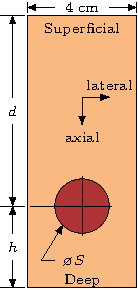
\includegraphics[width=0.9375in]{assets/quasistatic/drawings/schematic_single-crop.pdf}
				\label{fig:schematic_single}
			}
			~
			\subfloat[]{
				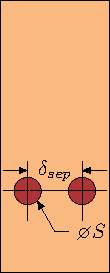
\includegraphics[width=0.7623625in]{assets/quasistatic/drawings/schematic_colocated-crop.pdf}
				\label{fig:schematic_colocated}
			}
			~
			\subfloat[]{
				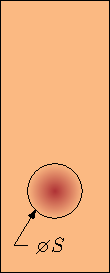
\includegraphics[width=0.7623625in]{assets/quasistatic/drawings/schematic_blur-crop.pdf}
				\label{fig:schematic_blur}
			}
			~
			\subfloat[]{
				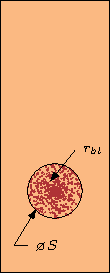
\includegraphics[width=0.7623625in]{assets/quasistatic/drawings/schematic_blob-crop.pdf}
				\label{fig:schematic_blob}
			}
			~
			\subfloat[]{
				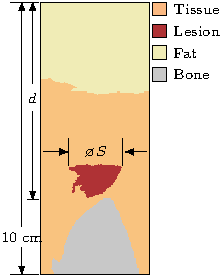
\includegraphics[width=1.4938125in]{assets/quasistatic/drawings/schematic_human-crop.pdf}
				\label{fig:schematic_human}
			}
			\caption[Quasi-static model geometries]{Model geometry showing the investigated lesions embedded in a \SI{4}{\cm} wide soft tissue domain. Axial and lateral directions mimic that of a typical ultrasound transducer placed along the top boundary of the domain. The simplest case of a circular lesion embedded in a soft tissue domain located superior to hard underlying bone is shown in \protect\subref{fig:schematic_single}. In order to investigate the interference caused by closely-located lesions, the case shown in \protect\subref{fig:schematic_colocated} was investigated. Because of the relatively unknown and variable geometric properties of deep tissue injury lesions, cases \protect\subref{fig:schematic_blur} and \protect\subref{fig:schematic_blob} were investigated where the lesion edges were blurred and the lesion was actually a large collection of small lesions, respectively. Finally, to investigate detection sensitivity in a realistic setting, case \protect\subref{fig:schematic_human} was investigated where an mri-acquired deep tissue injury was overlaid on a slice from the Visible Human Project such that the injury lesion was located immediately superior to an ischial tuberosity.}	
			\label{fig:geometry}
		\end{figure*}

		Simulated ultrasound images were acquired through the convolution of a point spread function with a normally distributed background map of scattering centres \cite{bamber80}. These images were then combined with a finite-element deformation model of the strained tissue to generate both pre- and post- compression images of the lesions and surrounding tissue. These images were fed into a tissue strain estimation algorithm to determine the detection sensitivity of the technique. Finally, the technique was validated against a physical phantom model using a subset of the simulated cases.

		\subsection{Formation of B-Mode Ultrasound Images}
			Through the convolution of a point spread function and a normal random distribution of scattering centres, simulated ultrasound images were generated. The point spread function was defined axially as a cosine function operating at the ultrasound probing frequency modulated by a Gaussian distribution defined by $\mu = 2\lambda$ and $\sigma = 2\lambda$ where $\lambda$ is the wavelength of the ultrasonic probing waves. Laterally, the point spread function was modelled as a Gaussian distribution defined by $\mu = 0$ and $\sigma = 0.25w_{active}$ where $w_{active}$ is the total width of the active transducer elements during scan-line acquisition.  This resulted in the point spread function given in Fig. \ref{fig:point_spread_function}. Resulting images were composed of 192 scan lines each sampled at \SI{50}{\MHz}.

			\begin{figure}[!t]
				\centering
					\begin{tikzpicture}
						\begin{axis}[
						width=0.75\textwidth,
						enlargelimits=false,
						unit vector ratio*=1 1 1,
						axis on top,
						xlabel={Lateral (\si{\mm})},
						ylabel={Axial (\si{\mm})},
						y dir=reverse,
						draw=black, text=black, fill=black
						]
							\addplot graphics[xmin=-1.15,xmax=1.15,ymin=0,ymax=1.54]{assets/quasistatic/images/psf.png};
						\end{axis}
					\end{tikzpicture}
				\caption[Point spread function used for simulating b-mode ultrasound scans]{Point spread function used for simulating b-mode ultrasound scans. The function is defined axially by a cosine function at the probing frequency and modulated by a Gaussian function both axially and laterally.}
				\label{fig:point_spread_function}
			\end{figure}

		\subsection{Finite-Element Model of Tissue Deformation Under Surface Distortion}
			As a response to an external load being applied to the boundary of a domain, internal structures deform. In the case of a relatively stiff deep tissue injury embedded within surrounding soft tissues, this implies that when the surface of the skin is depressed, the relatively stiff lesion will not strain to the same magnitude that the surrounding soft tissue does. In order to simulate the deformation of interrogated tissue, the displacement field for the simulated models was calculated according to:
			\begin{equation}
				- {\nabla} \cdot \sigma = {F}
			\end{equation}
			Where $\sigma$ is the Cauchy stress tensor and $F$ are the applied body forces. Simulations were performed assuming a 2-dimensional linearly elastic material deformation model under plane strain conditions. A 3-dimensional model was also considered, however the deformations differed from the 2-dimensional simulation by less than \SI{1}{\percent} so a 2-dimensional model was deemed adequate. Soft tissue was modelled using a Young's modulus of elasticity of \SI{25}{\kPa}, Poisson's ratio of 0.499, and density of \SI{998}{\kg\per\metre\cubed} \cite{krouskop98, choi05, martin94}. Bone was modelled in the Visible Human model with a Young's modulus of elasticity of \SI{18.6}{\GPa}, Poisson's ratio of 0.15 and density of \SI{297}{\kg\per\metre\cubed} \cite{rho93,shahar07,zheng00}. The only difference in lesion mechanical properties from the surrounding soft tissue was the modulus of elasticity which varied according to the simulation parameters. The bottom of the domain was held fixed such that:
			\begin{equation}
				{u} = 0, \qquad \Gamma = \Gamma_{bottom}
			\end{equation}
			While this boundary condition represents an idealized scenario, it may be likened to that of tissue located superficial to a relatively stiff anchoring bone below since the stiffness of bone is several orders of magnitude greater than soft tissue and will not significantly deform under the loads explored in this model. This lower region is where deep tissue injuries generally form and is therefore of special importance. Compressive strains were applied to the top of the domain so as to induce strain along the top boundary:
			\begin{equation}
				{u} = (0, -u_0), \qquad \Gamma = \Gamma_{top}
			\end{equation}

			From these simulations, displacement fields throughout the domain were calculated which were then used to displace tissue (including scattering centres) in the simulated ultrasound images in both the axial and lateral directions. This process resulted in pairs of pre- and post- compression simulated b-mode images of lesions of varying parameters which could then be analyzed and characterized.

		\subsection{Characterizing Quasi-Static Ultrasound Elastography}
			\label{sec:elastography_algorithm}
			Utilizing a 2-D locally regularized tissue strain estimation algorithm \cite{brusseau08}, pairs of pre- and post- compression images were used to calculate elastogram estimations for the full range of parameter values of the simulated lesions. The algorithm consists of sweeping the image domain with a series of overlapping regions of interest (ROI). ROI are compared between pre- and post- compression images, with ROI in the post- compression images being axially scaled and translated and laterally translated versions of the same ROI in the pre-compression images.

			Qualitatively, the noise and computation time of the resulting elastograms were found to be minimum when using an axial ROI size of approximately 10 times the ultrasound wavelength. Axial ROI overlap was held at \SI{99}{\percent} to produce elastograms with minimal noise, even though this introduced significant increases in computation time. Due to the extreme anisotropic nature of ultrasound signals, lateral ROI size was kept to 5 signal widths with lateral ROI overlaps of \SI{80}{\percent}.

		\subsection{Model Validation Using a Commercially Available Phantom}
			Utilizing a CIRS Elasticity QA Phantom model 049, a subset of the results obtained from the finite-element simulations and numerical characterizations were compared against their physical phantom equivalents. The phantom mimics acoustically homogeneous soft tissue with embedded lesions which vary in depth, size, and mechanical stiffness. Mechanical properties of the phantom as given by manufacturer specifications are summarized in Table \ref{tab:phantomproperties}. Pre- and post- compression b-mode ultrasound images were obtained of each lesion in the phantom and the resulting strain ratio for that lesion was compared to the simulated strain ratio for that combination of parameters. Specifically, lesions at a depth of \SI{3.5}{\cm}, a diameter of \SI{2.0}{\cm}, and with true stiffness ratios of 0.56, 1.80, and 3.20 were examined. Surface indentation was performed manually with the transducer indenting approximately \SI{0.5}{\cm} (\SI{6.25}{\percent}) at the surface.

			\begin{table}[!t]
				\centering
				\caption{CIRS Phantom Model Mechanical Properties}
				\label{tab:phantomproperties}
				\begin{tabular}{lcc}
					\toprule
					Property & Value \\
					\midrule
					Nominal basal stiffness & \SI{25}{\kPa} \\
					Lesion stiffness &  $[8, 14, 45, 80]$\,\si{\kPa} \\
					Speed of sound & \SI{1540}{\metre\per\second} \\
					Acoustic attenuation & \SI{0.5}{\decibel\per\cm\per\MHz} \\
					Lesion diameter & $[10, 20]$\,\si{\mm} \\
					Lesion depth & $[15, 35]$\,\si{\mm} \\
					\bottomrule
				\end{tabular}
			\end{table}

	\section{Results and Discussion}
		Following the procedure outlined in Section \ref{sec:method}, finite-element models of ultrasonic b-mode image formation and tissue deformation were synthesized. The results of these models were then fed into the local strain estimation algorithm described in Section \ref{sec:elastography_algorithm}. The resulting numerical characterizations of the relationship between measured and true strain ratios in the simulated tissue and their dependence on the various lesion parameters given in Table \ref{tab:parametervalues} were examined. Finally, the local strain estimation algorithm was carried out on a physical phantom and compared against a subset of the simulated cases.

		\subsection{Finite Element Models of Ultrasound and Deformation}
			\label{sec:femresults}
			Sample images generated using both the acoustic and deformation finite-element models are given in Figs. \ref{fig:precompression_bmode} -- \ref{fig:postcompression_bmode}. In Fig. \ref{fig:precompression_bmode}, a sample generated b-mode ultrasound scan is given. Fig. \ref{fig:displacement_field_u} shows the lateral displacement field generated by the deformation finite-element model while Fig. \ref{fig:displacement_field_v} shows the axial displacement field \note[KH]{Use colour images for displacement!}. The entire top surface of the model has been displaced axially by \SI{6.25}{\mm} (\SI{5}{\percent}), which caused deformation of both the soft tissue and embedded lesion within. Since the lesion was modelled as being 3.2 times stiffer than the surrounding tissue, the lesion underwent less strain which consequently resulted in the lesser displacement depicted. Fig. \ref{fig:postcompression_bmode} shows the resultant b-mode image generated by applying the displacement field given in Figs. \ref{fig:displacement_field_u} and \ref{fig:displacement_field_v} to the tissue and embedded scattering centres used to create Fig. \ref{fig:precompression_bmode}. What results is a locally scaled and translated version of Fig. \ref{fig:precompression_bmode} that corresponds to indenting the surface of the skin above a stiff lesion. The large anechoic region located at the bottom of the domain is tissue that was not modelled in the pre-compression image as it was outside of the original domain. This area represents the region of tissue that is undetectable with the strain-estimation algorithm given in Section \ref{sec:elastography_algorithm} as the information contained there is only available in one of the two input images and so is considered incomplete data.

			\addtocounter{footnote}{-1}
			\begin{figure*}[!t]
				\centering
				\subfloat[]{
					\begin{tikzpicture}
						\begin{axis}[width=0.6\textwidth, enlargelimits=false, unit vector ratio*=1 1 1, axis on top, xlabel={Lateral deviation, $x$ (\si{\cm})}, ylabel={}, y dir=reverse, colormap/blackwhite, colorbar, point meta min=-1.17, point meta max=1.17, colorbar style={at={(1.05,0)}, anchor=south west, width=0.01\textwidth, ylabel={Lateral Displacement (\si{\mm})},
						draw=black, text=black, fill=black},
						draw=black, text=black, fill=black]
							\addplot graphics[xmin=-2,xmax=2,ymin=0,ymax=12.5]{assets/quasistatic/images/displacement_u.png};
						\end{axis}
					\end{tikzpicture}
					\label{fig:displacement_field_u}
				}
				~
				\subfloat[]{
					\begin{tikzpicture}
						\begin{axis}[width=0.6\textwidth, enlargelimits=false, unit vector ratio*=1 1 1, axis on top, xlabel={Lateral deviation, $x$ (\si{\cm})}, ylabel={}, y dir=reverse, colormap={whiteblack}{gray(0cm)=(1); gray(1cm)=(0)}, colorbar, point meta min=-6.25, point meta max=0, colorbar style={at={(1.05,0)}, anchor=south west, width=0.01\textwidth, ylabel={Axial Displacement (\si{\mm})},
						draw=black, text=black, fill=black, y dir=reverse},
						draw=black, text=black, fill=black]
							\addplot graphics[xmin=-2,xmax=2,ymin=0,ymax=12.5]{assets/quasistatic/images/displacement_v.png};
						\end{axis}
					\end{tikzpicture}
					\label{fig:displacement_field_v}
				}
				
				\subfloat[]{
					\begin{tikzpicture}
						\begin{axis}[width=0.6\textwidth, enlargelimits=false, unit vector ratio*=1 1 1, axis on top, xlabel={Lateral deviation, $x$ (\si{\cm})}, ylabel={Depth, $d$ (\si{\cm})}, y dir=reverse,
						draw=black, text=black, fill=black]
							\addplot graphics[xmin=-2,xmax=2,ymin=0,ymax=12.5]{assets/quasistatic/images/bModeA.png};
						\end{axis}
					\end{tikzpicture}
					\label{fig:precompression_bmode}
				}
				~
				\subfloat[]{
					\begin{tikzpicture}
						\begin{axis}[width=0.6\textwidth, enlargelimits=false, unit vector ratio*=1 1 1, axis on top, xlabel={Lateral deviation, $x$ (\si{\cm})}, ylabel={Depth, $d$ (\si{\cm})}, y dir=reverse,
						draw=black, text=black, fill=black]
							\addplot graphics[xmin=-2,xmax=2,ymin=0,ymax=12.5]{assets/quasistatic/images/bModeB.png};
						\end{axis}
					\end{tikzpicture}
					\label{fig:postcompression_bmode}
				}
				\caption[Sample deformation finite-element model results for a hard spherical lesion]{Finite-element model results for the case when \ensuremath{d=\SI{10}{\cm}}, \ensuremath{\diameter S = \SI{2.5}{\cm}}, \ensuremath{\varepsilon_{rel} = 3.20}, and \ensuremath{f=\SI{4}{\MHz}} showing \protect\subref{fig:displacement_field_u} the lateral displacement field and \protect\subref{fig:displacement_field_v} the axial displacement field induced by compressive strain applied to the top of the boundary, \protect\subref{fig:precompression_bmode} a generated b-mode image of the pre-compressed tissue domain, and \protect\subref{fig:postcompression_bmode} a generated b-mode image of the post-compressed tissue domain. The included lesion is not visible in \protect\subref{fig:precompression_bmode} and \protect\subref{fig:postcompression_bmode} as it's acoustic properties were no different than surrounding tissues. An anechoic region is visible along the bottom of the domain in \protect\subref{fig:postcompression_bmode} which represents tissue outside of the domain visible in \protect\subref{fig:precompression_bmode}.}
				\label{fig:modelresults}
			\end{figure*}

		\subsection{Resulting Elastograms}
			\label{sec:elastogram}
			The 2-D locally regularized tissue strain estimation algorithm described in Section \ref{sec:elastography_algorithm} was used in combination with the simulated resultant b-mode ultrasound images (Figs. \ref{fig:precompression_bmode} and \ref{fig:postcompression_bmode}) in order to generate elastogram images which were used in the subsequent analysis. An example elastogram resulting from the simulation presented in Fig. \ref{fig:modelresults} is shown in Fig. \ref{fig:sample_elastogram}. Throughout the entire domain on this sample elastogram, regions outside of the stiff lesions showed compressive strains of approximately \SI{5}{\percent} as expected due to the compression applied to the upper boundary of the model. The entire lesion region showed relatively consistent low strain amounts of approximately \SI{2.5}{\percent}, which is consistent with the lesion being stiffer (and so straining less) than the surrounding tissue. Of note is the increased strain pattern which appeared both axially and laterally around the lesion. While generally symmetric about the axial direction, this stress field was largely concentrated above the lesion when the lesion was deep (close to the bone). This may be explained as a stress concentration brought about by the sudden change in mechanical material properties of the tissue and may serve to fuel the conditions of excessive cell deformation and ischemia which initiated the formation of a deep tissue injury in the first place, exacerbating the wound and assisting its expansion toward the surface. Further, a largely variable strain field artifact is seen along the superior surface of the elastogram shown in Fig. \ref{fig:sample_elastogram}. While this field does not appear to affect the remainder of the generated elastogram, it will serve to mask any extremely shallow legions in the tissue, though given as deep tissue injuries generally form immediately superior to boney prominences, this is unlikely to be the case. It is hypothesized that this variable strain field may be due to the large deformations present along the superior surface of the domain.

			\begin{figure}[!t]
				\centering
					\begin{tikzpicture}
						\begin{axis}[width=\columnwidth, enlargelimits=false, unit vector ratio*=1 1 1, axis on top, xlabel={Lateral deviation, $x$ (\si{\cm})}, ylabel={Depth, $d$ (\si{\cm})}, y dir=reverse, colormap/jet, colorbar, point meta min=0, point meta max=7, colorbar style={yticklabel={\pgfmathprintnumber{\tick}\,\percent},at={(1.05,0)}, width=0.01\textwidth, ylabel={Compressive Strain}, anchor=south west,
						draw=black, text=black, fill=black},
						draw=black, text=black, fill=black]
							\addplot graphics[xmin=-2,xmax=2,ymin=0,ymax=12.5]{assets/quasistatic/elastograms/e040_colour.png};
						\end{axis}
					\end{tikzpicture}
				\caption[Sample strain elastogram for a hard spherical lesion]{Sample strain elastogram showing estimated strain values for $d=\SI{10}{\cm}$, $\diameter S = \SI{2.5}{\cm}$, $\varepsilon_{rel} = 3.20$, $f = \SI{4}{\MHz}$. While undetectable on a single b-mode image, the elastogram clearly shows a low-strain (stiff) lesion located approximately \SI{10}{\cm} from the surface.}
				\label{fig:sample_elastogram}
			\end{figure}

		\subsection{Numerical Characterizations}
			\label{sec:numericalcharacterizations}
			In order to determine the sensitivity of using quasi-static ultrasound elastography to detect deep tissue injuries, elastograms such as the example that was calculated in Section \ref{sec:elastogram} were calculated for the full range of parameters given in Table \ref{tab:parametervalues}. ``Measured'' strain ratios for each elastogram were obtained by comparing the mean strain within each lesion with the mean engineering strain of the surrounding tissue such that:
			\begin{equation}
				\varepsilon_{rel,measured} = \frac{\varepsilon_{tissue}}{\varepsilon_{lesion}}
			\end{equation}

			$\varepsilon_{tissue}$ was sampled as the mean strain in the region of tissue with the same geometry as the lesion located immediately superficial to the lesion in all cases.

			In order to characterize how each parameter of interest affects the detection sensitivity of quasi-static ultrasound elastography, measured strain ratios for various lesions were calculated and compared against $\varepsilon_{rel,true}$. $\varepsilon_{rel,true}$ is derived from the relative Young's modulus of elasticity of the lesion such that:
			\begin{equation}
				\varepsilon_{rel,true} = \frac{\varepsilon_{tissue}}{\varepsilon_{lesion}} = \frac{\left(\frac{\sigma_{applied}}{E_{tissue}}\right)}{\left(\frac{\sigma_{applied}}{E_{lesion}}\right)} = \frac{E_{lesion}}{E_{tissue}}
			\end{equation}

			\begin{figure}[!t]
				\centering
				\begin{tikzpicture}
					\begin{axis}[
						scale only axis,
						height=3in,
						width=\textwidth-\widthof{100}-1in,
						xlabel={Lesion Stiffness Ratio},
						ylabel={\percent Error},
						grid=major,
						clip=true,
						cycle list name=ColourPlotCycle,
						draw=black, text=black, fill=black]
						\addplot+[error bars/.cd, y dir=both, y explicit, error bar style={ultra thick}] table[x index=0, y index=1, y error index=2] {assets/quasistatic/data/error_stiffness_ratio.dat};
					\end{axis}
				\end{tikzpicture}
				\caption[Detection ability as it is related to true lesion stiffness ratio]{Detection ability as it is related to true lesion stiffness ratio. For all but small lesion stiffness ratios (very soft ``lesions''), results are linear and predictable. For small lesion stiffness ratios (0.32), the lesion becomes severely misrepresented. This is likely due to the algorithm ``losing track'' of scattering centres for the relatively large displacements induced in the significantly less stiff tissue.}
				\label{fig:error_stiffness_ratio}
			\end{figure}

			Fig. \ref{fig:error_stiffness_ratio} portrays the severe error involved with using the methods described in Section \ref{sec:method} to investigate extremely low stiffness lesions. In nearly all investigated cases where the true lesion stiffness ratio was 0.32, the algorithms described severely misrepresented the measured strain ratio of the lesion, often portraying these extremely low stiffness regions as being more stiff than they truly were. It is hypothesized that the excessively large localized deformations in these lesions interrupted the algorithm's ability to sufficiently track the displacement of scattering centres within the tissue, lowering the magnitude of displacement within the lesion and subsequently increasing it's ``measured'' strain ratio.

			\begin{figure}[!t]
				\centering
				\begin{tikzpicture}
					\begin{axis}[
						scale only axis,
						height=3in,
						width=\textwidth-\widthof{100}-1in,
						xlabel={Normalized Characterization Index},
						ylabel={\percent Error},
						grid=major,
						legend entries={Lesion Size, Lesion Depth, Bone Separation, Probing Frequency, Applied Strain},
						legend style={at={(0.5,0.975)},anchor=north,font=\small},
						clip=true,
						cycle list name=ColourPlotCycle,
						ymax=70,
						draw=black, text=black, fill=black]
						\addplot table {assets/quasistatic/data/normalized_size.dat};
						\addplot table {assets/quasistatic/data/normalized_depth.dat};
						\addplot table {assets/quasistatic/data/normalized_bottomsep.dat};
						\addplot table {assets/quasistatic/data/normalized_frequency.dat};
						\addplot table {assets/quasistatic/data/normalized_strain.dat};
					\end{axis}
				\end{tikzpicture}
				\caption[Error characterization for a hard spherical lesion]{Error characterization for range of studied parameters for the simple model of a spherical lesion embedded within soft tissue as seen in Fig. \ref{fig:schematic_single}. Each parameter has been normalized to the range studied so overly-sensitive regions may be readily distinguished.}
				\label{fig:normalized_characterization}
			\end{figure}

			\begin{figure}[!t]
				\centering
				\begin{tikzpicture}
					\begin{axis}[
						scale only axis,
						height=3in,
						width=\textwidth-\widthof{100}-1in,
						xlabel={Normalized Characterization Index},
						ylabel={\percent Error},
						grid=major,
						legend entries={Boundary Blur Radius, Co-Located Lesion Separation, Clustered Lesion Density, Clustered Lesion Size, Human Lesion Size, Human Lesion Depth},
						legend style={legend pos=north east,font=\small},
						clip=true,
						cycle list name=ColourPlotCycle,
						ymax=80,
						draw=black, text=black, fill=black]
						\addplot table {assets/quasistatic/data/normalized_lesion_sep.dat};
						\addplot table {assets/quasistatic/data/normalized_blur_radius.dat};
						\addplot table {assets/quasistatic/data/normalized_blob_density.dat};
						\addplot table {assets/quasistatic/data/normalized_blob_radius.dat};
						\addplot table {assets/quasistatic/data/normalized_human_size.dat};
						\addplot table {assets/quasistatic/data/normalized_human_depth.dat};
					\end{axis}
				\end{tikzpicture}
				\caption[Error characterization for: co-located, blurred boundary, clustered, and visible human lesion models]{Error characterization for range of studied parameters for the co-located lesions, blurred boundary lesions, clustered lesions, and visible human lesion models as seen in Figs. \ref{fig:schematic_colocated} -- \ref{fig:schematic_human}. Each parameter has been normalized to the range studied so overly-sensitive regions may be readily distinguished.}
				\label{fig:normalized_characterization_extras}
			\end{figure}

			In order to broadly investigate the critical parameter-values of the investigated models, each parameter was normalized to its investigated range and the error resulting over these ranges is given in Figs. \ref{fig:normalized_characterization} and \ref{fig:normalized_characterization_extras}.

			In Fig. \ref{fig:normalized_characterization}, it is clear to see that the most sensitive error-inducing situations occur when either the lesion is very small or if large strains are used to deform the tissue. Similarly, it is expected that if the lesion depth were increased much further, significant errors would arise with increasing depth. Logically, this may be explained due to the decreasing magnitude of displacement with increasing depth---at a certain point, the magnitude of displacement of scattering centres will be on par with the measurement noise, and the lesion will cease to be detectable.

			From Fig. \ref{fig:normalized_characterization_extras} it can be seen that small lesions in the Visible Human-MRI model as well as co-located lesions with large separation distances produce greater measurement errors. Conversely, lesion depth in the Visible Human-MRI model; lesion density and individual lesion size in the clustered lesion model; and boundary blur radius in the blurred-edges model do not seem to affect the measurement error significantly. Of note is the relative large amount of static error present in the boundary blur radius model which is hypothesized to be due to lesser mean tissue stiffness in the investigated region than expected.

			\begin{figure}[!t]
				\centering
				\begin{tikzpicture}
					\begin{axis}[
						scale only axis,
						height=3in,
						width=\textwidth-\widthof{100}-1in,
						xlabel={True Lesion Stiffness Ratio, $E_{true}$},
						ylabel={Measured Lesion Stiffness Ratio, $E_{meas}$},
						grid=major,
						legend entries={$\diameter S = \SI{0.5}{\cm}$, $\diameter S = \SI{1.0}{\cm}$, $\diameter S = \SI{2.0}{\cm}$, $\diameter S = \SI{2.5}{\cm}$},
						legend style={legend pos=north west,font=\small},
						clip=true,
						cycle list name=ColourPlotCycle,
						draw=black, text=black, fill=black]
						\addplot table {assets/quasistatic/data/circular_size_05.dat};
						\addplot table {assets/quasistatic/data/circular_size_10.dat};
						\addplot table {assets/quasistatic/data/circular_size_20.dat};
						\addplot table {assets/quasistatic/data/circular_size_25.dat};
						\node [anchor=south](c) at (axis cs:3.125,0.6) {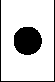
\includegraphics{assets/quasistatic/insets/inset_single.pdf}};
					\end{axis}
				\end{tikzpicture}
				\caption[Quasi-static lesion size characterization]{Lesion size characterization at a depth of \SI{10}{\cm} with a \SI{4}{\MHz} ultrasound probing frequency showing increasing detection sensitivity of the lesion with increasing lesion size. Detection sensitivity is less than ideal for all cases, with the best case being for lesions approximately \SI{2.5}{\cm} in diameter.}
				\label{fig:size_characterization}
			\end{figure}

			Fig. \ref{fig:size_characterization} shows the relationship between lesion size and detection sensitivity for lesions at a depth of \SI{10}{\cm} in a model depth of \SI{12.5}{\cm} interrogated at \SI{4}{\MHz} with \SI{5}{\percent} applied strain. Specifically, Fig. \ref{fig:size_characterization} shows the decreasing detection sensitivity with decreasing lesion size with the best detection sensitivity being with the largest investigated lesions with a diameter of \SI{2.5}{\cm}. On the opposite end, the detection sensitivity of lesions at or below \SI{0.5}{\cm} in diameter is questionable. Although data is lacking on the true size of formative DTI, MRI results indicate that untreated DTI are on the scale of multiple centimetres \cite{solis13}. Thus, the ability to detect lesions of at least \SI{1}{\cm} in diameter should prove to be adequate to both detect and monitor DTI.

			In order to investigate the effect of lesion depth on the detection sensitivity, measured strain ratios for circular lesions with a diameter of \SI{2.5}{\cm} located at various depths were interrogated with a \SI{4}{\MHz} probing frequency, and strained by \SI{5}{\percent}. The results of this investigation are seen in Fig. \ref{fig:depth_characterization}.

			\begin{figure}[!t]
				\centering
				\begin{tikzpicture}
					\begin{axis}[
						scale only axis,
						height=3in,
						width=\textwidth-\widthof{100}-1in,
						xlabel={True Lesion Stiffness Ratio, $E_{true}$},
						ylabel={Measured Lesion Stiffness Ratio, $E_{meas}$},
						grid=major,
						legend entries={$d = \SI{3.5}{\cm}$, $d = \SI{6.5}{\cm}$, $d = \SI{8.5}{\cm}$, $d = \SI{10}{\cm}$},
						legend style={legend pos=north west,font=\small},
						clip=true,
						cycle list name=ColourPlotCycle,
						draw=black, text=black, fill=black]
						\addplot table {assets/quasistatic/data/circular_depth_035.dat};
						\addplot table {assets/quasistatic/data/circular_depth_065.dat};
						\addplot table {assets/quasistatic/data/circular_depth_085.dat};
						\addplot table {assets/quasistatic/data/circular_depth_100.dat};
						\node [anchor=south](c) at (axis cs:3.125,0.6) {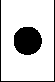
\includegraphics{assets/quasistatic/insets/inset_single.pdf}};
					\end{axis}
				\end{tikzpicture}
				\caption[Quasi-static lesion depth characterization]{Lesion depth characterization at a lesion diameter of \SI{2.5}{\cm} with a \SI{4}{\MHz} ultrasound probing frequency generally showing general independence of detection sensitivity on lesion depth in the tissue.}
				\label{fig:depth_characterization}
			\end{figure}

			In Fig. \ref{fig:depth_characterization}, it can be seen that there was little interplay between detection sensitivity and measured strain ratios at the various depths examined for all but the case for very soft (mushy) lesions (with a stiffness ratio of 0.32). At such low stiffness ratios, the excessive tissue deformation interrupts the tissue strain estimation algorithm's ability to adequately track the induced displacements in the lesion.

			Since the strain field caused by compressive forces near an extremely rigid structure embedded within a relatively soft domain will be significantly heterogeneous, the effect of lesion altitude above the underlying stiff bone was examined with the hypothesis that if the lesion were too close to the hard bone, it would be masked by the strain field caused by the bone's existence. A \SI{2.5}{\cm} diameter lesion was interrogated with a \SI{4}{\MHz} probing frequency and \SI{5}{\percent} applied strain. The results of this characterization are given in Fig. \ref{fig:bottomsep_characterization}.

			\begin{figure}[!t]
				\centering
				\begin{tikzpicture}
					\begin{axis}[
						scale only axis,
						height=3in,
						width=\textwidth-\widthof{100}-1in,
						xlabel={True Lesion Stiffness Ratio, $E_{true}$},
						ylabel={Measured Lesion Stiffness Ratio, $E_{meas}$},
						grid=major,
						legend entries={$h = \SI{1.25}{\cm}$, $h = \SI{2.50}{\cm}$, $h = \SI{3.75}{\cm}$},
						legend style={legend pos=north west,font=\small},
						clip=true,
						cycle list name=ColourPlotCycle,
						draw=black, text=black, fill=black]
						\addplot table {assets/quasistatic/data/circular_bottomsep_000.dat};
						\addplot table {assets/quasistatic/data/circular_bottomsep_125.dat};
						\addplot table {assets/quasistatic/data/circular_bottomsep_250.dat};
						\node [anchor=south](c) at (axis cs:3.125,0.6) {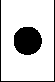
\includegraphics{assets/quasistatic/insets/inset_single.pdf}};
					\end{axis}
				\end{tikzpicture}
				\caption[Quasi-static lesion altitude characterization]{Effect of lesion altitude above the underlying bone. Aside from erroneous results at very low lesion stiffness ratios, the effect is negligible.}
				\label{fig:bottomsep_characterization}
			\end{figure}

			In Fig. \ref{fig:bottomsep_characterization}, it can be seen that the lesion altitude above the underlying bone had very little effect on the detection sensitivity. Although larger strain fields may be generated near the bone, it is hypothesized that the larger fields also extend larger and so affect healthy tissue to more or less the same degree as the forming lesion.

			In order to characterize the effect of using alternate ultrasound probing frequencies, simulations were carried out on lesions using probing frequencies of \SI{2}{\MHz}, \SI{4}{\MHz}, and \SI{8}{\MHz}. The simulated lesions had a diameter of \SI{2.5}{\cm}, were located at a depth of \SI{10}{\cm} and we strain at \SI{5}{\percent}. The results of this study are given in Fig. \ref{fig:freq_characterization}.

			\begin{figure}[!t]
				\centering
				\begin{tikzpicture}
					\begin{axis}[
						scale only axis,
						height=3in,
						width=\textwidth-\widthof{100}-1in,
						xlabel={True Lesion Stiffness Ratio, $E_{true}$},
						ylabel={Measured Lesion Stiffness Ratio, $E_{meas}$},
						grid=major,
						legend entries={$f = \SI{2}{\MHz}$, $f = \SI{4}{\MHz}$, $f = \SI{8}{\MHz}$},
						legend style={legend pos=north west,font=\small},
						clip=true,
						cycle list name=ColourPlotCycle,
						draw=black, text=black, fill=black]
						\addplot table {assets/quasistatic/data/circular_frequency_2.dat};
						\addplot table {assets/quasistatic/data/circular_frequency_4.dat};
						\addplot table {assets/quasistatic/data/circular_frequency_8.dat};
						\node [anchor=south](c) at (axis cs:3.125,0.55) {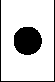
\includegraphics{assets/quasistatic/insets/inset_single.pdf}};
					\end{axis}
				\end{tikzpicture}
				\caption[Quasi-static ultrasound probing frequency characterization]{Characterization of ultrasonic probing frequency on detection sensitivity. Apart from the requirement of using an ultrasonic frequency low enough to interrogate the desired tissue, probing frequency has negligible effect on the detection sensitivity.}
				\label{fig:freq_characterization}
			\end{figure}

			As can be seen from Fig. \ref{fig:freq_characterization}, there is very little effect on the detection sensitivity from the ultrasound probing frequency that was used, therefore an appropriate frequency should be chosen so as to reach the the full depth of the bone-muscle interface at suspected DTI locations while retaining the best image resolution.

			As quasi-static ultrasound elastography is most likely to be performed via manual indentation where the exact magnitude of applied deformation is unknown, it is important to study the effect of applied strain magnitude on the detection sensitivity. Applied strains of \SI{2.5}{\percent}, \SI{5.0}{\percent}, and \SI{10}{\percent} were investigated on a \SI{2.5}{\cm} diameter lesion at a depth of \SI{10}{\cm} using a probing frequency of \SI{4}{\MHz}; the results are given in Fig. \ref{fig:strain_characterization}.

			\begin{figure}[!t]
				\centering
				\begin{tikzpicture}
					\begin{axis}[
						scale only axis,
						height=3in,
						width=\textwidth-\widthof{100}-1in,
						xlabel={True Lesion Stiffness Ratio, $E_{true}$},
						ylabel={Measured Lesion Stiffness Ratio, $E_{meas}$},
						grid=major,
						legend entries={$\varepsilon_{app} = \SI{2.5}{\percent}$, $\varepsilon_{app} = \SI{5.0}{\percent}$, $\varepsilon_{app} = \SI{10.0}{\percent}$},
						legend style={legend pos=north west,font=\small},
						clip=true,
						cycle list name=ColourPlotCycle,
						draw=black, text=black, fill=black]
						\addplot table {assets/quasistatic/data/circular_strain_025.dat};
						\addplot table {assets/quasistatic/data/circular_strain_050.dat};
						\addplot table {assets/quasistatic/data/circular_strain_100.dat};
						\node [anchor=south](c) at (axis cs:3.125,0.6) {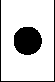
\includegraphics{assets/quasistatic/insets/inset_single.pdf}};
					\end{axis}
				\end{tikzpicture}
				\caption[Quasi-static applied strain characterization]{Applied strain characterization plot for lesions with a diamater of \SI{2.5}{\cm} located at a depth of \SI{10}{\cm} interrogated at \SI{4}{\MHz}. There is little difference between \SI{2.5}{\percent} and \SI{5.0}{\percent} applied strain, while large-magnitude strains of \SI{10}{\percent} generate significant error for both very soft and very stiff lesions.}
				\label{fig:strain_characterization}
			\end{figure}

			While Fig. \ref{fig:strain_characterization} shows a relatively constant detection sensitivity for compressive strains of \SI{2.5}{\percent} and \SI{5}{\percent}, compressive strains of \SI{10}{\percent} generate significant measurement error for both very soft and very stiff lesions. Under large compressive strains, the tissue (either in the lesion as in the soft lesion case, or the surrounding tissue as in the stiff lesion case) deforms considerably which again interferes with the algorithm's ability to properly track the displacement of tissue. It should also be noted that applying overly large strains to an already forming deep tissue injury may cause additional unwarranted damage. Thus it is imperative that applied surface indentation be kept to reasonable bounds (\SI{2.5}{\percent} -- \SI{5}{\percent}, or \SI{0.25}{\cm} -- \SI{0.50}{\cm} in \SI{10}{\cm} deep domains), not only for safety of the tissue but also for clarity of the diagnostic test.

			To study the effect that closely spaced lesions will have on the detection sensitivity as well as how discernible the lesions will be from each other, the separation distance between two \SI{1.0}{\cm} diameter co-located lesions at a depth of \SI{10}{\cm} was examined using a \SI{4}{\MHz} probing frequency with \SI{5}{\percent} applied strain magnitude. The results of this study are shown in \ref{fig:separation_characterization}.

			\begin{figure}[!t]
				\centering
				\begin{tikzpicture}
					\begin{axis}[
						scale only axis,
						height=3in,
						width=\textwidth-\widthof{100}-1in,
						xlabel={True Lesion Stiffness Ratio, $E_{true}$},
						ylabel={Measured Lesion Stiffness Ratio, $E_{meas}$},
						grid=major,
						legend entries={$\delta_{sep} = \SI{1.25}{\cm}$, $\delta_{sep} = \SI{1.50}{\cm}$, $\delta_{sep} = \SI{1.75}{\cm}$, $\delta_{sep} = \SI{2.00}{\cm}$},
						legend style={legend pos=north west,font=\small},
						clip=true,
						cycle list name=ColourPlotCycle,
						draw=black, text=black, fill=black]
							\addplot table {assets/quasistatic/data/separation_0125.dat};
							\addplot table {assets/quasistatic/data/separation_0150.dat};
							\addplot table {assets/quasistatic/data/separation_0175.dat};
							\addplot table {assets/quasistatic/data/separation_0200.dat};
							\node [anchor=south](c) at (axis cs:3.125,0.7) {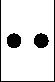
\includegraphics{assets/quasistatic/insets/inset_colocated.pdf}};
					\end{axis}
				\end{tikzpicture}
				\caption[Quasi-static lesion separation distance characterization]{Effect of lesion separation distance on two \SI{1.0}{\cm} diameter lesions co-located at a depth of \SI{10}{\cm} interrogated with a \SI{4}{\MHz} probe with \SI{5}{\percent} applied strain. There is no negligible difference between separation distances on the detection sensitivity.}
				\label{fig:separation_characterization}
			\end{figure}

			While Fig. \ref{fig:separation_characterization} shows that the separation distance between co-located lesions causes a negligible effect on the detection sensitivity, Fig. \ref{fig:separation_elastogram} shows regions of decreased strain above and below the centreline of the lesions. While these regions had the same basal stiffness as the bulk tissue, the decreased strain pattern may obfuscate the true results by introducing ``phantom lesions'' which are not actually present but merely the result of the existing lesions.

			\begin{figure}[!t]
				\centering
				\begin{tikzpicture}
					\begin{axis}[
						width=\columnwidth,
						enlargelimits=false,
						unit vector ratio*=1 1 1,
						axis on top,
						xlabel={Lateral deviation, $x$ (\si{\cm})},
						ylabel={Depth, $d$ (\si{\cm})},
						y dir=reverse,
						colormap/jet,
						colorbar,
						point meta min=0,
						point meta max=7,
						colorbar style={yticklabel={\pgfmathprintnumber{\tick}\,\si{\percent}}, at={(1.05,0)}, width=0.01\textwidth, ylabel={Compressive Strain}, anchor=south west,
						draw=black, text=black, fill=black},
						draw=black, text=black, fill=black]
							\addplot graphics[xmin=-2,xmax=2,ymin=0,ymax=12.5]{assets/quasistatic/elastograms/e080_colour.png};
					\end{axis}
				\end{tikzpicture}
				\caption[Sample elastogram for two co-located lesions]{Elastogram for two co-located lesions of \SI{1.0}{\cm} diameter at a depth of \SI{10}{\cm} interrogated using a \SI{4}{\MHz} probing frequency with \SI{5}{\percent} applied strain. A pattern of decreased strain is present above and below the centerline between the two lesions while the lesions themselves are not affected by each other.}
				\label{fig:separation_elastogram}
			\end{figure}

			While the simulations performed thus far assumed that lesions were perfect spheres with hard boundaries in order to isolate specific parameters of interest, this assumption may not always be accurate. Rather, due to the nature of injury formation, lesions may form gradual boundaries that ``fade'' from stiff or necrotic tissue to healthy tissue. To investigate the effect of this phenomenon on the detection sensitivity, lesions with ``blurred boundaries'' were investigated. Hard spherical lesions were blurred by convolving the lesion domain with a disc blurring kernel of varying radius. The results for this investigation on lesions with a diameter of \SI{2.5}{\cm}, at a depth of \SI{10}{\cm} and interrogated with a \SI{4}{\MHz} probing frequency with \SI{5}{\percent} applied strain are given in Fig. \ref{fig:blur_radius_characterization}.

			\begin{figure}[!t]
				\centering
				\begin{tikzpicture}
					\begin{axis}[
						scale only axis,
						height=3in,
						width=\textwidth-\widthof{100}-1in,
						xlabel={True Lesion Stiffness Ratio, $E_{true}$},
						ylabel={Measured Lesion Stiffness Ratio, $E_{meas}$},
						grid=major,
						legend entries={$b_r = \SI{1.0}{\mm}$, $b_r = \SI{2.5}{\mm}$, $b_r = \SI{5.0}{\mm}$, $b_r = \SI{7.5}{\mm}$},
						legend style={legend pos=north west,font=\small},
						clip=true,
						cycle list name=ColourPlotCycle,
						draw=black, text=black, fill=black
						]
							\addplot table {assets/quasistatic/data/blur_radius_01.dat};
							\addplot table {assets/quasistatic/data/blur_radius_25.dat};
							\addplot table {assets/quasistatic/data/blur_radius_50.dat};
							\addplot table {assets/quasistatic/data/blur_radius_75.dat};
							\node [anchor=south](c) at (axis cs:3.125,0.6) {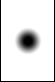
\includegraphics{assets/quasistatic/insets/inset_blur.pdf}};
					\end{axis}
				\end{tikzpicture}
				\caption[Quasi-static lesion blur radius characterization]{Characterization of the effect of lesion blur radius on lesion detection sensitivity for a \SI{2.5}{\cm} diameter lesion at a depth of \SI{10}{\cm} using a probing frequency of \SI{4}{\MHz} and applied strain of \SI{5}{\percent}. While there is negligible effect of the blur radius on stiff lesions, the strain ratio for soft lesions is considerably over-estimated.}
				\label{fig:blur_radius_characterization}
			\end{figure}

			Fig. \ref{fig:blur_radius_characterization} shows that there is very little dependence on the lesion detection sensitivity for stiff lesions (lesions with a stiffness ratio $\geq 1.0$). However, for soft lesions, the tissue strain estimation algorithm seems to over-estimate the stiffness of the lesions.

			% REASON?

			Similar to how lesions may have ``blurred boundaries'' rather that hard ones, so too may lesion composition not be homogeneous. In order to study the effect of heterogeneous regions of injured tissue, the detection sensitivity of a set of numerous small lesions located within close proximity to each other so as to form a large, heterogeneous area of diseased tissue was examined. Fig. \ref{fig:blob_density_characterization} shows the results for this model for varying numbers of \SI{2}{\mm} diameter lesions in a \SI{2.5}{\cm} diameter circle located at a depth of \SI{10}{\cm} with a probing frequency of \SI{4}{\MHz} and \SI{5}{\percent} applied strain. Fig. \ref{fig:blob_radius_characterization} further explores this model by investigating the case where there are 30 small lesions per square \SI{}{\cm} with individual lesions ranging in diameter from \SI{0.5}{\mm} to \SI{1.5}{\mm}.

			\begin{figure}[!t]
				\centering
				\begin{tikzpicture}
					\begin{axis}[
						scale only axis,
						height=3in,
						width=\textwidth-\widthof{100}-1in,
						xlabel={True Lesion Stiffness Ratio, $E_{true}$},
						ylabel={Measured Lesion Stiffness Ratio, $E_{meas}$},
						grid=major,
						legend entries={$b_\rho = \SI[per=reciprocal]{10}{\per\cm\squared}$, $b_\rho = \SI[per=reciprocal]{20}{\per\cm\squared}$, $b_\rho = \SI[per=reciprocal]{30}{\per\cm\squared}$, $b_\rho = \SI[per=reciprocal]{40}{\per\cm\squared}$},
						legend style={legend pos=north west,font=\small},
						clip=true,
						cycle list name=ColourPlotCycle,
						draw=black, text=black, fill=black]
							\addplot table {assets/quasistatic/data/blob_density_10.dat};
							\addplot table {assets/quasistatic/data/blob_density_20.dat};
							\addplot table {assets/quasistatic/data/blob_density_30.dat};
							\addplot table {assets/quasistatic/data/blob_density_40.dat};
							\node [anchor=south](c) at (axis cs:3.125,0.6) {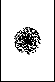
\includegraphics{assets/quasistatic/insets/inset_blob.pdf}};
					\end{axis}
				\end{tikzpicture}
				\caption[Quasi-static lesion density characterization]{Characterization of lesion density for a group of numerous smaller \SI{2}{\mm} diameter lesions comprising a large area with a diameter of \SI{2.5}{\cm} at a depth of \SI{10}{\cm} interrogated with a \SI{4}{\MHz} probing frequency and \SI{5}{\percent} applied strain. Detection sensitivity decreases with decreasing lesion density, as expected.}
				\label{fig:blob_density_characterization}
			\end{figure}

			The characterization plot in Fig. \ref{fig:blob_density_characterization} for small lesion density is less linear than other characterization plots, with lesion density having a significant effect on the detection sensitivity. Specifically, for low lesion densities, the detection sensitivity is much lower than for high lesion densities. However, this observation is warranted after examination of the elastogram produced from these results, given in Fig. \ref{fig:blob_elastogram}, which shows how the small lesions are not individually detected but rather the entire region is detected as one large lesion. Since the average stiffness ratio over this region is lesser than the stiffness ratio of individual lesions, it makes sense that the ``measured'' strain ratio will be less than expected.

			\begin{figure}[!t]
				\centering
				\subfloat[]{
					\begin{tikzpicture}
						\begin{axis}[
							width=0.9\columnwidth,
							enlargelimits=false,
							unit vector ratio*=1 1 1,
							axis on top,
							xlabel={Lateral deviation, $x$ (\si{\cm})},
							ylabel={Depth, $d$ (\si{\cm})},
							y dir=reverse,
							draw=black, text=black, fill=black]
								\addplot graphics[xmin=-2,xmax=2,ymin=0,ymax=12.5]{assets/quasistatic/images/stiffnessMap_092_colour.png};
						\end{axis}
					\end{tikzpicture}
					\label{fig:blob_elastogram_a}
				}
				~
				\subfloat[]{
					\begin{tikzpicture}
						\begin{axis}[
							width=0.9\columnwidth,
							enlargelimits=false,
							unit vector ratio*=1 1 1,
							axis on top,
							xlabel={Lateral deviation, $x$ (\si{\cm})},
							ylabel={Depth, $d$ (\si{\cm})},
							y dir=reverse,
							colormap/jet,
							colorbar,
							point meta min=0,
							point meta max=7,
							colorbar style={yticklabel={\pgfmathprintnumber{\tick}\,\si{\percent}}, at={(1.05,0)}, width=0.01\textwidth, ylabel={Compressive Strain}, anchor=south west,
							draw=black, text=black, fill=black},
							draw=black, text=black, fill=black]
								\addplot graphics[xmin=-2,xmax=2,ymin=0,ymax=12.5]{assets/quasistatic/elastograms/e092_colour.png};
						\end{axis}
					\end{tikzpicture}
					\label{fig:blob_elastogram_b}
				}
				\caption[Sample elastogram for a set of clustered lesions]{Stiffness map \protect\subref{fig:blob_elastogram_a} and corresponding elastogram \protect\subref{fig:blob_elastogram_b} for a group a small lesions with a density of 10 lesions per \SI{}{cm^2} grouped in a \SI{2.5}{\cm} diameter circle at a depth of \SI{10}{\cm} interrogated with a \SI{4}{\MHz} probing frequency and \SI{5}{\percent} applied strain. In \protect\subref{fig:blob_elastogram_a}, white regions are regular tissue while black regions are the small lesions. In the elastogram, individual lesions do not stand out, rather the entire region of lesions appears as one large region of unhealthy tissue.}
				\label{fig:blob_elastogram}
			\end{figure}

			\begin{figure}[!t]
				\centering
				\begin{tikzpicture}
					\begin{axis}[
						scale only axis,
						height=3in,
						width=\textwidth-\widthof{100}-1in,
						xlabel={True Lesion Stiffness Ratio, $E_{true}$},
						ylabel={Measured Lesion Stiffness Ratio, $E_{meas}$},
						grid=major,
						legend entries={$r_{bl} = \SI{0.5}{\mm}$, $r_{bl} = \SI{1.0}{\mm}$, $r_{bl} = \SI{2.0}{\mm}$, $r_{bl} = \SI{2.5}{\mm}$},
						legend style={legend pos=north west,font=\small},
						clip=true,
						cycle list name=ColourPlotCycle,
						draw=black, text=black, fill=black]
							\addplot table {assets/quasistatic/data/blob_radius_05.dat};
							\addplot table {assets/quasistatic/data/blob_radius_10.dat};
							\addplot table {assets/quasistatic/data/blob_radius_15.dat};
							\node [anchor=south](c) at (axis cs:3.125,0.6) {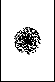
\includegraphics{assets/quasistatic/insets/inset_blob.pdf}};
					\end{axis}
				\end{tikzpicture}
				\caption[Quasi-static clustered lesion radius characterization]{Characterization of lesion radius for a group of numerous smaller lesions with a density of 30 lesions per \SI{}{cm^2} comprising a large area with a diameter of \SI{2.5}{\cm} at a depth of \SI{10}{\cm} interrogated with a \SI{4}{\MHz} probing frequency and \SI{5}{\percent} applied strain. Detection sensitivity decreases with decreasing individual lesion size, as expected.}
				\label{fig:blob_radius_characterization}
			\end{figure}

			Similar to the results shown in Fig. \ref{fig:blob_density_characterization}, changing the size of the individual small lesions does have an effect on the measured strain. In this case, when individual lesions are small, the total area occupied by lesions is lesser which results in a lesser average tissue stiffness over the grouped lesion region.

			Note that although the elastography algorithm was able to detect the larger lesion-filled regions in these simulations, it was completely unable to discern the individual lesions comprising those regions. This is not surprising due to both the generated strain fields in the healthy tissue throughout the larger lesion area as well as the results presented in Fig. \ref{fig:size_characterization} showing poor detection sensitivity for lesions with diameters $\leq \SI{1}{\cm}$ while the individual lesions in this simulation had diameters of the scale of \SI{0.5}{\mm} -- \SI{1.5}{\mm}.

			Finally, in order to place these results within the context of a likely real scenario in humans, a more complicated model utilizing an MRI-acquired lesion and slides from the Visible Human Project \cite{visiblehuman} was developed. Specifically, lesion geometry was taken from a real deep tissue injury in a pig model imaged using $\mathrm{T}_2^*$-weighted MRI. The human geometry was taken from a transverse plane slice aross the left ischial tuberosity such that the lesion was placed immediately superficial to the boney promience. For this model, the overall lesion width and lesion depth were examined with results shown in Figs. \ref{fig:human_size_characterization} and \ref{fig:human_depth_characterization} respectively.

			\begin{figure}[!t]
				\centering
				\begin{tikzpicture}
					\begin{axis}[
						scale only axis,
						height=3in,
						width=\textwidth-\widthof{100}-1in,
						xlabel={True Lesion Stiffness Ratio, $E_{true}$},
						ylabel={Measured Lesion Stiffness Ratio, $E_{meas}$},
						grid=major,
						legend entries={$\diameter S = \SI{0.5}{\cm}$, $\diameter S = \SI{1.0}{\cm}$, $\diameter S = \SI{2.0}{\cm}$, $\diameter S = \SI{2.5}{\cm}$},
						legend style={legend pos=north west,font=\small},
						clip=true,
						cycle list name=ColourPlotCycle,
						draw=black, text=black, fill=black]
							\addplot table {assets/quasistatic/data/human_size_05.dat};
							\addplot table {assets/quasistatic/data/human_size_10.dat};
							\addplot table {assets/quasistatic/data/human_size_20.dat};
							\addplot table {assets/quasistatic/data/human_size_25.dat};
							\node [anchor=south](c) at (axis cs:3.2,0.7) {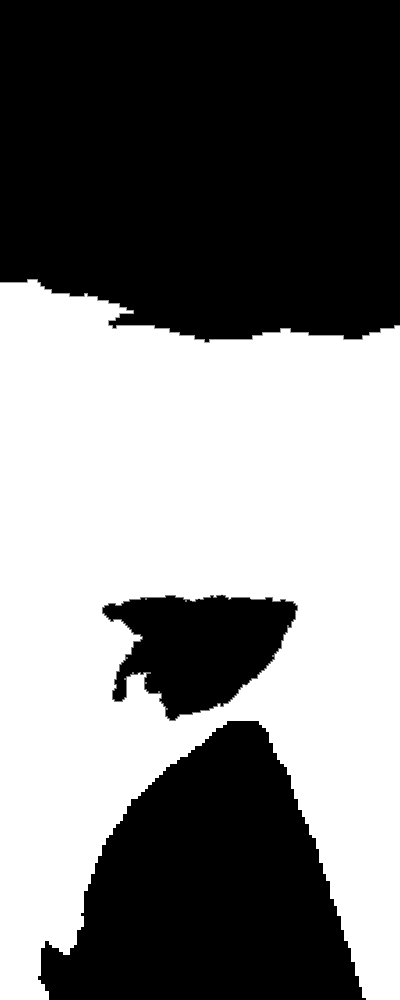
\includegraphics[width=0.072\columnwidth]{assets/quasistatic/insets/human.png}};
							\node [anchor=south](rect) at (axis cs:3.2,0.72) [draw,minimum width=0.072\columnwidth,minimum height=0.18\columnwidth]{};
					\end{axis}
				\end{tikzpicture}
				\caption[Quasi-static Visible Human model lesion width characterization]{Characterization of lesion width in a Visible Human-MRI model for lesions at a depth of \SI{7.25}{\cm} interrogated with a \SI{4}{\MHz} probing frequency with \SI{5}{\percent} applied strain. Small lesions (with a width $\leq \SI{1.0}{\cm}$) are severely misrepresented and portray general over-estimation of lesion stiffness larger lesions.}
				\label{fig:human_size_characterization}
			\end{figure}

			In Fig. \ref{fig:human_size_characterization}, it is clear to see than small lesions (with a diameter $\leq \SI{1.0}{\cm}$) are almost impossible to adequately detect (although larger lesions will be adequately detectable). It is hypothesized that this phenomenon is due to the excessive strain apparent above the boney prominence that is seen in the resultant elastogram given in Fig. \ref{fig:human_elastogram} such that the lesion is ``washed out'' by the strain field developed by the relatively stiff bone nearby.

			\begin{figure}[!t]
				\centering
				\begin{tikzpicture}
					\begin{axis}[
						width=\columnwidth,
						enlargelimits=false,
						unit vector ratio*=1 1 1,
						axis on top,
						xlabel={Lateral deviation, $x$ (\si{\cm})},
						ylabel={Depth, $d$ (\si{\cm})},
						y dir=reverse,
						colormap/jet,
						colorbar,
						point meta min=0,
						point meta max=7,
						colorbar style={yticklabel={\pgfmathprintnumber{\tick}\,\si{\percent}}, at={(1.05,0)}, width=0.01\textwidth, ylabel={Compressive Strain}, anchor=south west,
						draw=black, text=black, fill=black},
						draw=black, text=black, fill=black]
							\addplot graphics[xmin=-2,xmax=2,ymin=0,ymax=10]{assets/quasistatic/elastograms/e117_colour.png};
					\end{axis}
				\end{tikzpicture}
				\caption[Sample elastogram of a Visible Human model lesion]{Elastogram for a \SI{0.5}{\cm} wide lesion embedded in the Visible Human-MRI model domain at a depth of \SI{7.25}{\cm} interrogated at \SI{4}{\MHz} with an applied strain of \SI{2.5}{\percent}. The lesion is not visible in the resultant elastogram.}
				\label{fig:human_elastogram}
			\end{figure}

			\begin{figure}[!t]
				\centering
				\begin{tikzpicture}
					\begin{axis}[
						scale only axis,
						height=3in,
						width=\textwidth-\widthof{100}-1in,
						xlabel={True Lesion Stiffness Ratio, $E_{true}$},
						ylabel={Measured Lesion Stiffness Ratio, $E_{meas}$},
						grid=major,
						legend entries={$d = \SI{6.25}{\cm}$, $d = \SI{6.75}{\cm}$, $d = \SI{7.25}{\cm}$},
						legend style={legend pos=north west,font=\small},
						clip=true,
						cycle list name=ColourPlotCycle,
						draw=black, text=black, fill=black]
							\addplot table {assets/quasistatic/data/human_bottom_sep_625.dat};
							\addplot table {assets/quasistatic/data/human_bottom_sep_675.dat};
							\addplot table {assets/quasistatic/data/human_bottom_sep_725.dat};
							\node [anchor=south](c) at (axis cs:3.2,0.62) {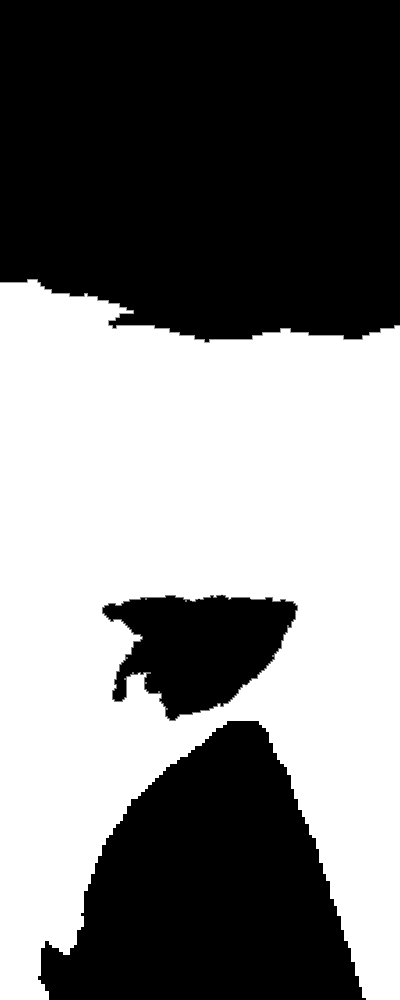
\includegraphics[width=0.072\columnwidth]{assets/quasistatic/insets/human.png}};
							\node [anchor=south](rect) at (axis cs:3.2,0.64) [draw,minimum width=0.072\columnwidth,minimum height=0.18\columnwidth]{};
					\end{axis}
				\end{tikzpicture}
				\caption[Quasi-static characterization of lesion depth in a Visible Human model]{Characterization of lesion depth in a Visible Human-MRI model for lesions with a width of \SI{2.5}{\cm} interrogated with a \SI{4}{\MHz} probing frequency and \SI{5}{\percent} applied strain. Deeper lesions (closer to the bony promience) are have slightly over-estimated lesion stiffness ratios as opposed to more superficial lesions while detection sensitivity is not affected by lesion depth.}
				\label{fig:human_depth_characterization}
			\end{figure}

			In Fig. \ref{fig:human_depth_characterization}, there is little to no dependence of the detection sensitivity on the lesion depth in the Visible Human-MRI model with all depth curves displaying the same profile. However, deeper lesions (lesions closer to the bony prominence) have stiffnesses that are over-estimated with respect to their superficial counterparts. This is hypothesized to be due to the increased strain field present in all of the soft tissue located immediately superior to the bony prominence, but should not pose a serious problem for imaging lesions of this nature.

		\subsection{Physical Phantom Validation}
			In order to ensure that the models presented here represented physical realities, a small subset of the cases studied were modelled in a physical phantom, specifically for three lesions with stiffness ratios of 0.56, 1.80, and 3.20 with a diameter of \SI{2.0}{\cm} and at a depth of \SI{3.5}{\cm}, interrogated at \SI{8}{\MHz} with approximately \SI{5}{\percent} applied strain. The results of this study are summarized in Fig. \ref{fig:phantom_validation}.

			\begin{figure}[!t]
				\centering
				\begin{tikzpicture}
					\begin{axis}[
						scale only axis,
						height=3in,
						width=\textwidth-\widthof{100}-1in,
						xlabel={Simulated Measured Strain Ratio, $E_{sim,measured}$},
						ylabel style={align=center},
						ylabel={Experimental Measured \\ Stiffness Ratio, $E_{exp,measured}$},
						legend entries={Results, Ideal},
						legend style={legend pos=south east,font=\small},grid=major,clip=true,cycle list name=ColourPlotCycle,
						xmin=0.5, xmax=2.5,
						ymin=0.5, ymax=2.5,
						draw=black, text=black, fill=black]
							\addplot[mark=none,dashed,ultra thick] table {assets/quasistatic/data/ideal_1_1.dat};
							\addplot table {assets/quasistatic/data/validation.dat};
							\node [anchor=north west](c) at (axis cs:0.55,2.45) {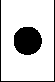
\includegraphics{assets/quasistatic/insets/inset_single.pdf}};
					\end{axis}
				\end{tikzpicture}
				\caption[Experimental validation of quasi-static model results]{Relation between simulated measured strain ratios and experimental measured strain ratios for a lesion at a depth of \SI{3.5}{\cm} and diameter of \SI{2.0}{\cm} showing general agreement between simulated and experimental cases. Idealization errors are the most likely the cause of the differences seen between simulated and experimental cases.}
				\label{fig:phantom_validation}
			\end{figure}

			As can be seen in Fig. \ref{fig:phantom_validation}, a relatively simple (although inexact) relationship between simulated and experimental measured strain ratios exists. It must be noted that the finite-element simulations of b-mode image formation and tissue deformation presented here are idealizations of reality and idealization errors such as the ultrasound pulse profile and plane-strain assumption no doubt contributed to the difference seen in Fig. \ref{fig:phantom_validation}.

			It must be noted that in order to acquire quasi-static elastography results in the physical phantom, the ultrasound transducer was required to be manually manipulated to cause indentation in the phantom, as the technique would most likely be performed in a clinical setting. This was found to be problematic as the ultrasound transducer was difficult to maintain perfectly perpendicular and in-plane during the compression (largely due to the necessity of using coupling ultrasonic gel). This difficulty suggests that acoustic radiation force impulse (ARFI) elastography would be a more appropriate method to acquire DTI elastograms. ARFI elastography works on the same principles as quasi-static elastography with the exception that tissue deformation is caused by localized large-amplitude acoustic waves generated by the transducer such that human factors play a far less substantial role in image acquisition.

	\section{Conclusion}
		With this work, we presented a numerical characterization of the use of quasi-static ultrasound elastography for the early detection of deep tissue injuries (DTI). There is a real clinical need for an objective tool that is capable of detecting the formation and progression of DTI in human subjects as these wounds are generally not visible from the surface of the skin until they have broken through and already caused substantial damage.

		Through our numerical characterization, quasi-static ultrasound elastography was found to be an effective tool for detecting and monitoring DTI in theoretical simulations. Overall, detection sensitivity was less than expected. Small lesions (with diameters $\leq \SI{1.0}{\cm}$) were more difficult to differentiate due to the low lesion detection sensitivity. While lesion depth, altitude above the underlying bone, and probing frequency did not have significant effect on the lesion detection sensitivity, it was found that applying high levels of compressive strain (\SI{10}{\percent}) introduced severe error for both very soft and very stiff lesions, thus it is recommended that diagnosticians only apply moderate ($\leq \SI{5}{\percent}$) compressive strain when interrogating potential lesions. Larger strains may alternately be induced by slowly palpating the tissue with very minor strains frame-by-frame and cumulating the displacement fields across these smaller palpations. Care must be used when palpating the tissue, lest ``vigorous'' palpations cause harm to the already sensitive injury. In the more complicated model of co-located lesions, while the separation distance between adjacent lesions did not affect the detection sensitivity, the placing of adjacent lesions generated ``phantom'' lesion regions with altered strain that may appear to be diseased tissue when they are in fact healthy. In a model lesion with gradual blurred boundaries, the effect of blur radius only affected the detection sensitivity and ability to differentiate soft lesions. Specifically, soft lesions with large blur radii became nearly impossible to differentiate as these lesions all showed a measured lesion stiffness ratio of approximately 1 which would show up as regular, healthy tissue. In the case of numerous clustered small lesions, both decreased lesion density and decreased individual lesion size caused a decrease in lesion detection sensitivity, likely due to the averaging effect of healthy tissue and diseased tissue in near proximity. Finally, in the Visible Human-MRI acquired lesion model, lesions with widths $\leq \SI{1.0}{\cm}$ are nearly impossible to differentiate as they are hidden by the strain field generated by the bony prominence. Lesion depth did not have an effect on the detection sensitivity, though deeper lesions (lesions which were closer to the bony prominence) had overestimated stiffnesses with respect to their more superficial counterparts.

		Although the studies presented here resulted in less-than-ideal detection sensitivities, the technique was still able to pick out lesions from the surrounding soft (and hard) tissue. Work done by Solis et al. \cite{solis13} has shown that untreated DTI are multiple centimeters in size, while work done by Gefen et al. \cite{gefen05} has shown that deep tissue injuries exhibit 1.8-fold to 3.3-fold mechanical stiffening. The work presented here has shown that quasi-static ultrasound elastography is adequate at detecting deep tissue injury lesions in these ranges of parameters and will thus be adequate to detect and monitor progress DTI. However, without further real-world experimentation on the exact nature of newly-forming DTI, the detection sensitivity required to detect newly-forming DTI is indeterminate.

		A subset of the results found through simulation were compared with similar experiments done using a tissue mimicking phantom model. The experimental results using the phantom model generally agreed with those found from simulation cases. It was also noted that the manual skin indentation technique involved with quasi-static ultrasound elastography proved to be difficult to produce reliable images. This difficulty suggests that an alternate method of performing ultrasound elastography may be preferable to quasi-static ultrasound elastography with manual indentation. Acoustic radiation force impulse (ARFI) elastography may be a more appropriate method to acquire DTI elastograms as although ARFI elastography works on the same principles as quasi-static elastography, the difference lays in the fact that tissue deformation is caused by localized large-amplitude acoustic waves generated by the transducer. This means that human factors play a far less substantial role in image acquisition and would likely improve repeatability and inter-operator reliability. Nevertheless, the work done here to characterize the use of quasi-static ultrasound elastography is an important step along the path of generating a useful clinical tool for detecting formative and monitoring progressive deep tissue injuries.

\comment{
	\cleardoublepage

	\phantomsection

	\addcontentsline{toc}{section}{References}
	\bibcomplete{references}
	\printbibliography[heading=subbibliography]
}